%================2.1
\section{Bài toán phân loại hai lớp}

Bài toán phân loại hai lớp (hai quần thể), ký hiệu là $C_1$ và $C_2$, là một trong những trường hợp cơ bản và quan trọng nhất của nhận dạng mẫu thống kê. Nội dung phần này trình bày chi tiết cách xây dựng quy tắc phân loại tối ưu cho hai lớp dựa trên nền tảng lý thuyết đã thiết lập ở Chương 1, đặc biệt là sự gặp gỡ nội tại giữa tiêu chuẩn chiếu tối ưu hình học của Fisher và lý thuyết quyết định Bayes dưới mô hình phân phối chuẩn.

\subsection{Thiết lập bài toán và giả thiết mô hình xác suất}

Xét đối tượng cần phân loại được biểu diễn bởi vectơ đặc trưng $X = x \in \mathbb{R}^d$. Bài toán quyết định lớp của $x$ được xây dựng trên các nền tảng sau:
\begin{itemize}
    \item \textbf{Xác suất tiên nghiệm (Prior probability):} Ký hiệu xác suất đối tượng thuộc về lớp $C_1$ là $P(C_1)$ và thuộc lớp $C_2$ là $P(C_2)$, với điều kiện $P(C_1) + P(C_2) = 1$.
    \item \textbf{Mật độ có điều kiện (Likelihood):} Mỗi lớp tuân theo một phân phối chuẩn $d$ chiều (Gaussian) và giả thiết hai lớp có chung một cấu trúc ma trận hiệp phương sai $\Sigma$:
    \begin{equation}
        X | C_k \sim N_d(\mu_k, \Sigma) \quad \text{với } k = 1, 2.
    \end{equation}
    Hàm mật độ của $X$ khi biết lớp $C_k$ là: $p(x | C_k) = \frac{1}{(2\pi)^{d/2} |\Sigma|^{1/2}} \exp\left\{ -\frac{1}{2}(x - \mu_k)^T \Sigma^{-1} (x - \mu_k) \right\}$.
    \item \textbf{Ma trận hàm tổn thất (Loss Matrix):} Để đánh giá hệ quả của việc sai lầm, ta thiết lập ma trận tổn thất $L = \begin{pmatrix} 0 & L_{12} \\ L_{21} & 0 \end{pmatrix}$. Trong đó, $L_{ij}$ là chi phí rủi ro khi quyết định đối tượng thuộc lớp $C_j$ nhưng thực tế đối tượng lại thuộc về lớp $C_i$.
\end{itemize}

\subsection{Quy tắc phân loại Bayes cho bài toán hai lớp}

Theo lý thuyết quyết định Bayes, để cực tiểu hóa rủi ro kỳ vọng hậu nghiệm, ta đánh giá giá trị rủi ro có điều kiện tại $x$. Quy tắc tối ưu sẽ ưu tiên đưa đối tượng vào nhóm $C_1$ (chọn hành động $a_1$) nếu $R(a_1|x) < R(a_2|x)$. Với cấu trúc ma trận tổn thất định trước, điều kiện này tương đương với:
\begin{equation}
    L_{21} P(C_2 | x) < L_{12} P(C_1 | x) \iff \frac{P(C_1 | x)}{P(C_2 | x)} > \frac{L_{21}}{L_{12}}
\end{equation}
Áp dụng định lý Bayes, ta chuyển về bất phương trình logarit của tỷ số hợp lý:
\begin{equation}
    \ln \frac{p(x | C_1)}{p(x | C_2)} + \ln \frac{L_{12} P(C_1)}{L_{21} P(C_2)} > 0
\end{equation}
Tại đây, nhờ giả thiết hai lớp có cùng ma trận hiệp phương sai ($\Sigma_1 = \Sigma_2 = \Sigma$), các thành phần bậc hai của $x$ triệt tiêu. Phương trình thu gọn còn lại là một hàm phân tách tuyến tính (Dichotomic function) ký hiệu là $D(x)$:
\begin{equation}
    D(x) = (\mu_1 - \mu_2)^T \Sigma^{-1} x - \frac{1}{2}\left( \mu_1^T \Sigma^{-1} \mu_1 - \mu_2^T \Sigma^{-1} \mu_2 \right) + C
\end{equation}
trong đó đặt $C = \ln \frac{L_{12} P(C_1)}{L_{21} P(C_2)}$. 
Bằng việc nhóm các định thức tương ứng liên quan, ta có thể viết lại $D(x)$ dưới dạng trung tâm:
\begin{equation}\label{eq:bayes_rule_two_class}
    D(x) = (\mu_1 - \mu_2)^T \Sigma^{-1} \left( x - \frac{\mu_1 + \mu_2}{2} \right) + C
\end{equation}

Tóm lại, \textbf{Quy tắc quyết định Bayes đa biến} trong bài toán hai lớp là: Nếu $D(x) > 0$, ta phân loại đối tượng $x$ vào nhóm $C_1$, và ngược lại vào nhóm $C_2$.

\subsection{Sự giao thoa và tương đương với tiếp cận của Fisher}

Nhìn lại thuật toán Linear Discriminant Analysis của Fisher, hướng chiếu không gian giúp dữ liệu phân tách tối ưu nhất chính là:
\begin{equation}
    \beta^* = \Sigma^{-1}(\mu_1 - \mu_2)
\end{equation}
Nếu áp dụng phương pháp Fisher vào hàm phân biệt $D(x)$ tại phương trình (\ref{eq:bayes_rule_two_class}), ta có:
\begin{equation}
    D(x) = \beta^{*T} \left( x - \frac{\mu_1 + \mu_2}{2} \right) + C
\end{equation}

Trong kịch bản cân bằng, khi các lỗi bị xử phạt đối xứng ($L_{12} = L_{21}$) và xác suất tiên nghiệm giữa các lớp bằng nhau ($P(C_1) = P(C_2)$), hằng số tổn thất tiên nghiệm $C = 0$. Khi ấy hàm $D(x) > 0$ có thể biểu diễn qua hệ bất phương trình:
\begin{equation}
    \beta^{*T} x > \beta^{*T} \frac{\mu_1 + \mu_2}{2} \iff y > y_0
\end{equation}
trong đó $y = \beta^{*T} x$ là giá trị hình chiếu 1 chiều tự nhiên của quan sát $x$, và $y_0 = \frac{\beta^{*T} \mu_1 + \beta^{*T} \mu_2}{2}$ là trung điểm (ngưỡng cắt) giữa hai trung bình sau khi chiếu. 

Như vậy, mô hình quyết định theo phân phối chuẩn đồng hiệp phương sai của Bayes dẫn trực tiếp đến tiêu chuẩn phân loại hình học thông qua hướng chiếu tối ưu Fisher. Phép chiếu $\beta^*$ kết hợp với ngưỡng chia ở trung điểm thực tế là quy tắc phân cực tự nhiên của thống kê và lý thuyết.

\subsection{Thủ tục Bayes Classifier trong thực nghiệm}

Trong ngữ cảnh thực tiễn, do sự thiếu khuyết của tham số tổng thể ($\mu_1, \mu_2, \Sigma, P(C_k)$), hệ thống phân loại sẽ hoàn toàn sử dụng dữ liệu để dự báo thông qua các ước lượng mẫu:
\begin{itemize}
    \item \textbf{Input:} Tập huấn luyện $n$ điểm dữ liệu $\mathcal{D} = \{(x_i, y_i)\}_{i=1}^n$, gộp thành hai nhóm dữ liệu $D_1$ (cỡ $n_1$) và $D_2$ (cỡ $n_2$).
    
    \item \textbf{Bước 1: Tính các ước lượng tham số}
    Trung bình mẫu của từng lớp:
    \begin{equation}
        m_k = \frac{1}{n_k} \sum_{x \in D_k} x \quad (k=1, 2)
    \end{equation}
    Ma trận hiệp phương sai mẫu gộp $S_p$ (Pooled Sample Covariance Matrix) sẽ đóng vai trò là ước lượng không chệch cho $\Sigma$:
    \begin{equation}
        S_p = \frac{(n_1 - 1)S_1 + (n_2 - 1)S_2}{n - 2}
    \end{equation}
    với $S_k$ là hiệp phương sai tự nhiên của từng nhóm. Tỷ lệ phân phối tiên nghiệm sẽ được tính $\hat{P}(C_k) = \frac{n_k}{n}$.
    
    \item \textbf{Bước 2: Tìm hướng chiếu và ngưỡng quyết định} 
    Dựa trên quy luật Bayes được thực nghiệm hóa:
    \begin{equation}
        b_{opt} = S_p^{-1}(m_1 - m_2)
    \end{equation}
    Hàm phân biệt $\widehat{D}(x)$ đối với quan sát mới $x$ mang hình hài:
    \begin{equation}
        \widehat{D}(x) = b_{opt}^T \left( x - \frac{m_1 + m_2}{2} \right) + \widehat{C}
    \end{equation}
    với hạng tử tự do $\widehat{C} = \ln \frac{L_{12} n_1}{L_{21} n_2}$.
    
    \item \textbf{Bước 3: Phân loại đối tượng} 
    Áp dụng luật quyết định thực nghiệm: $\widehat{D}(x) > 0 \implies \text{quyết định } \widehat{G}(x) = C_1$. Ngược lại, xếp vào lớp $C_2$. Độ tin cậy và chất lượng của mô hình này sẽ được minh hoạ thông qua hàm rủi ro thực nghiệm trên tập mẫu (Empirical Risk).
\end{itemize}

\subsection{Ví dụ minh họa: Bài toán phân loại một chiều}

Để trực quan hóa lý thuyết trên, xét một ví dụ thực tiễn đơn giản trong không gian một chiều ($d=1$). Giả sử ta cần phân loại hai loại táo dựa trên một đặc trưng duy nhất là khối lượng $x$ (đơn vị: gram). Hai loại táo là:
\begin{itemize}
    \item Lớp $C_1$ (Táo xuất khẩu): Khối lượng trung bình $\mu_1 = 150\text{g}$.
    \item Lớp $C_2$ (Táo nội địa): Khối lượng trung bình $\mu_2 = 120\text{g}$.
\end{itemize}
Giả thiết rằng khối lượng của cả hai loại táo đều tuân theo phân phối chuẩn với cùng một phương sai $\sigma^2 = 100$ (độ lệch chuẩn $\sigma = 10\text{g}$). 

Với bài toán một chiều, ma trận nghịch đảo $\Sigma^{-1}$ tiêu biến thành $1/\sigma^2$. Hàm phân biệt Bayes theo dạng rút gọn tại bề mặt một chiều trở thành:
\begin{equation}
    D(x) = \frac{\mu_1 - \mu_2}{\sigma^2} \left( x - \frac{\mu_1 + \mu_2}{2} \right) + \ln \frac{L_{12} P(C_1)}{L_{21} P(C_2)}
\end{equation}

\textbf{Trường hợp 1 (Điều kiện cân bằng):} 
Giả định số lượng hai loại táo trên dây chuyền là như nhau ($P(C_1) = P(C_2) = 0.5$) và tổn thất do phân loại nhầm là ngang bẳng ($L_{12} = L_{21} = 1$). Hằng số tổn thất sinh ra giá trị $C = \ln(1) = 0$. Quy tắc quyết định $D(x) > 0$ phụ thuộc mặt toán học. Vì tỷ số $\frac{\mu_1 - \mu_2}{\sigma^2} = \frac{30}{100} > 0$, điều kiện phân loại rút gọn lại về phía ngưỡng bề mặt:
\begin{equation}
     x > \frac{\mu_1 + \mu_2}{2} \iff x > \frac{150 + 120}{2} = 135 \text{g}
\end{equation}
Như vậy, tất cả những quả táo nặng trên 135g sẽ được dán nhãn là Táo xuất khẩu ($C_1$), bằng hoặc dưới 135g là Táo nội địa ($C_2$).

\textbf{Trường hợp 2 (Sự bất đối xứng trong xác suất tiên nghiệm):} 
Giả sử trên thực tế, Táo nội địa chiếm thị phần với tỷ lệ sản lượng 80\% ($P(C_2) = 0.8$), trong khi Táo xuất khẩu hiếm hơn chỉ có 20\% ($P(C_1) = 0.2$). Vẫn giữ nguyên giả thiết mức phạt rủi ro đồng đều.
Khi đó, thành tố thiên lệch khoảng cách điểm mù $C \neq 0$ diễn ra:
\begin{equation}
    C = \ln \frac{1 \times 0.2}{1 \times 0.8} = \ln(0.25) \approx -1.386
\end{equation}
Hàm $D(x)$ nhận dạng mới là:
\begin{equation}
    D(x) = \frac{150 - 120}{100} (x - 135) - 1.386 = 0.3(x - 135) - 1.386 
\end{equation}
Quy tắc phân loại mới yêu cầu $D(x) > 0$:
\begin{equation}
    0.3(x - 135) > 1.386 \iff x > 135 + \frac{1.386}{0.3} = 139.62 \text{g}
\end{equation}
Trong tình huống ưu tiên Bayes tổng quát này, chỉ những quả táo thực sự khá nặng (hầu hết trên 139.62g) mới được xếp dòng thành Táo xuất khẩu $C_1$. Đường biên phân định đã bị dịch về phía của các táo thông thường. Lý tưởng về mặt logic của định lý Bayes muốn truyền đạt là: do Táo nội địa chiếm đa số, ta cần một bằng chứng quan sát mạnh mẽ (trọng lượng rất lớn) để bù đắp lại rủi ro về mặt xác xuất tiên nghiệm.

\subsection{Ví dụ minh họa: Bài toán phân loại hai chiều (Mô phỏng)}

Tiếp nối bài toán một chiều, ta xét một trường hợp tổng quát hơn trong không gian hai chiều ($d=2$). Thay vì sử dụng bộ dữ liệu có sẵn, ta tiến hành sinh mẫu ngẫu nhiên nhân tạo trong ngôn ngữ R để minh họa trực quan sự phân tách không gian của Fisher LDA theo phân phối chuẩn. 

\textbf{Thiết lập tham số sinh dữ liệu:}
\begin{itemize}
    \item Lớp $C_1$: Tập hợp gồm $n_1 = 500$ điểm dữ liệu được lấy mẫu ngẫu nhiên từ phân phối chuẩn đa biến $N_2(\mu_1, \Sigma)$. Vector trung bình $\mu_1 = (3, 3)^T$.
    \item Lớp $C_2$: Tập hợp gồm $n_2 = 500$ điểm dữ liệu được lấy mẫu ngẫu nhiên từ phân phối chuẩn đa biến $N_2(\mu_2, \Sigma)$. Vector trung bình $\mu_2 = (4, 4)^T$.
    \item Ma trận hiệp phương sai chung cho cả hai lớp (giả thiết cùng phương sai): 
    $$ \Sigma = \begin{pmatrix} 2 & -1.5 \\ -1.5 & 2 \end{pmatrix} $$
\end{itemize}

Do kích thước mẫu cân bằng ($n_1 = n_2 = 500$), tỷ lệ tiên nghiệm thực nghiệm trong mẫu là $\hat{P}(C_1) = \hat{P}(C_2) = 0.5$. Hằng số ngưỡng $C$ xấp xỉ bằng $0$.
Theo cơ chế học của đường phân tách tuyến tính Fisher, thuật toán tính toán ma trận tán xạ chung trong nội bộ nhóm ($S_w$), sau đó thiết lập vector pháp tuyến (vector hình chiếu tối ưu) làm đường biên tuyến tính. Kết quả phân bố trên không gian hai chiều và đường phân tách được minh họa trong Hình \ref{fig:2d_normal_class}.

\begin{figure}[!ht]
    \centering
    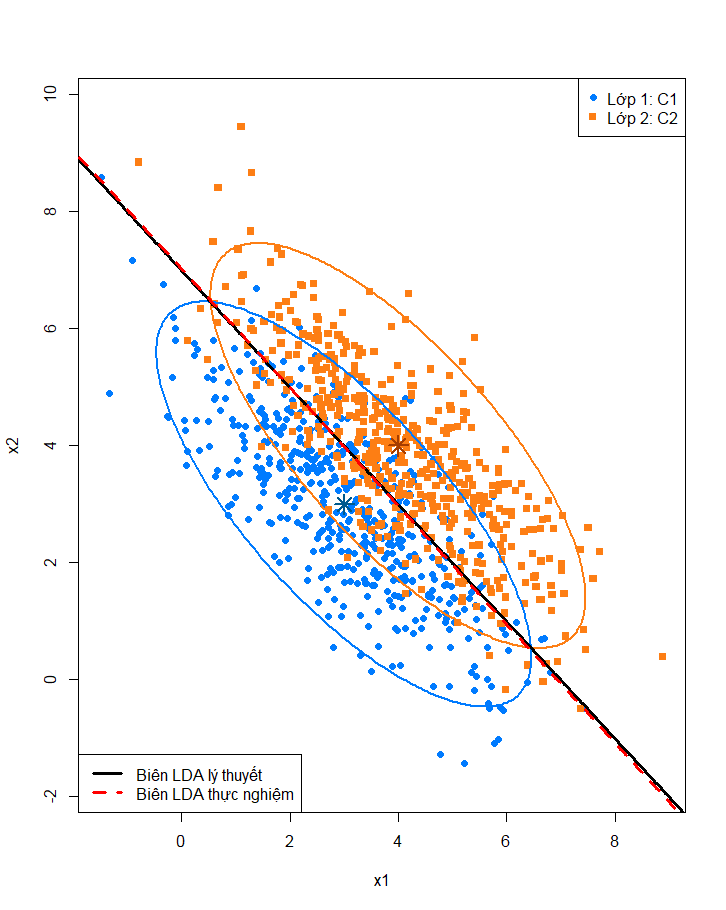
\includegraphics[width=0.8\textwidth]{image/normal_dis_2_classes.png}
    \caption{Phân bố mẫu của hai nhóm sinh từ phân phối chuẩn 2 chiều và đường phân loại sắc nét (Linear Decision Boundary) được xây dựng bởi giải thuật LDA.}
    \label{fig:2d_normal_class}
\end{figure}

Dựa trên hình vẽ \ref{fig:2d_normal_class}, các điểm dữ liệu đại diện cho hai nhóm có xu hướng thuôn giãn chéo góc do tồn tại sự tương quan âm trong ma trận $\Sigma$ ($\sigma_{12} = -1.5 < 0$). Đường ranh giới bình phương tối thiểu (LDA) cắt trực diện qua trung điểm giữa hai tâm $\mu_1$ và $\mu_2$, chia cắt không gian làm hai vùng dữ liệu hoàn hảo. Các đường mức hình ellipse bao quanh từng tâm xác nhận lại cấu trúc mật độ chuẩn Gaussian của dữ liệu đầu vào.

Để đánh giá định lượng chất lượng phân loại thực nghiệm của phương pháp này trên chính tập dữ liệu vừa sinh ra, ta áp dụng dự đoán nhãn cho toàn bộ $1000$ điểm mẫu từ mô hình LDA và lập Ma trận nhầm lẫn (Confusion Matrix).

\begin{figure}[!ht]
    \centering
    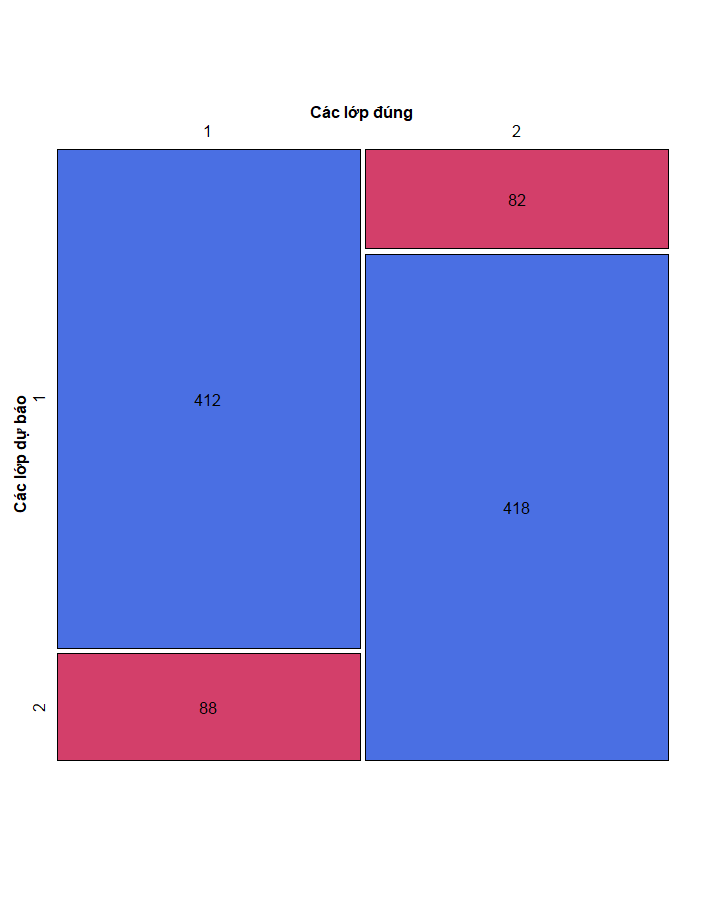
\includegraphics[width=0.6\textwidth]{image/confusion_matrix.png}
    \caption{Ma trận nhập nhằng (Confusion Matrix) dùng trong việc đánh giá mức độ chính xác của bộ phân lớp Fisher dựa trên đường thẳng tách biên.}
    \label{fig:confusion_matrix_lda}
\end{figure}

Hình \ref{fig:confusion_matrix_lda} cho thấy sự đan chéo đối chiếu giữa dự đoán từ lớp phân mảnh (Predicted Class) và nhãn gốc của mẫu sinh ngẫu nhiên ban đầu (Actual Class). Nhờ thuật toán tìm kiếm được đường biên phân chia hình học tối ưu nhất, lượng điểm rơi ngẫu nhiên vào miền sai lầm (False Positive và False Negative) là nhỏ tương đối so với phần lớn quần thể dự đoán trúng xác thực (True Positive và True Negative). Trong cấu trúc lớp này, do khoảng cách Mahalanobis giữa hai tập đủ lớn so với phương sai phân tán, sai số phân loại toàn cục (Error Rate) ở mức kiểm soát được một cách chặt chẽ. Điều này là minh chứng thực tế cho sự đồng điệu và hiệu suất đáng tin cậy giữa Tiêu chuẩn Fisher và Tiêu chuẩn cực tiểu hóa sai số Bayes.